\subsubsection{Spielmodi speziell}

Die verschiedenen Spielmodi wurden mittels eines von uns als Simulator bezeichneten Programms entwickelt und ausprobiert. So konnten wir u.a. prüfen, ob die Spielmodi wie erwartet funktionieren und ob bei realistischen Eingaben (also entsprechenden Schusswechseln zwischen den Spielern) Szenarien auftreten können, die entsprechend der Bedeutung des jeweiligen Spielmodus nicht sinnvoll sind. \\
Der Simulator ist kommandozeilenbasiert. Er ermöglicht alle wichtigen Eingaben, die im fertigen Produkt über die Website möglich sein sollten, u.a. der gewünschte Spielmodus, die Anzahl der Spieler, die Anzahl der zu spielenden Runden und die Unverwundbarkeitszeit. Lediglich Spielernamen kennt der Simulator nicht. Die simulierten Spieler werden einfach von 0 beginnend durchnummeriert. \\
\begin{figure}
  \centering
  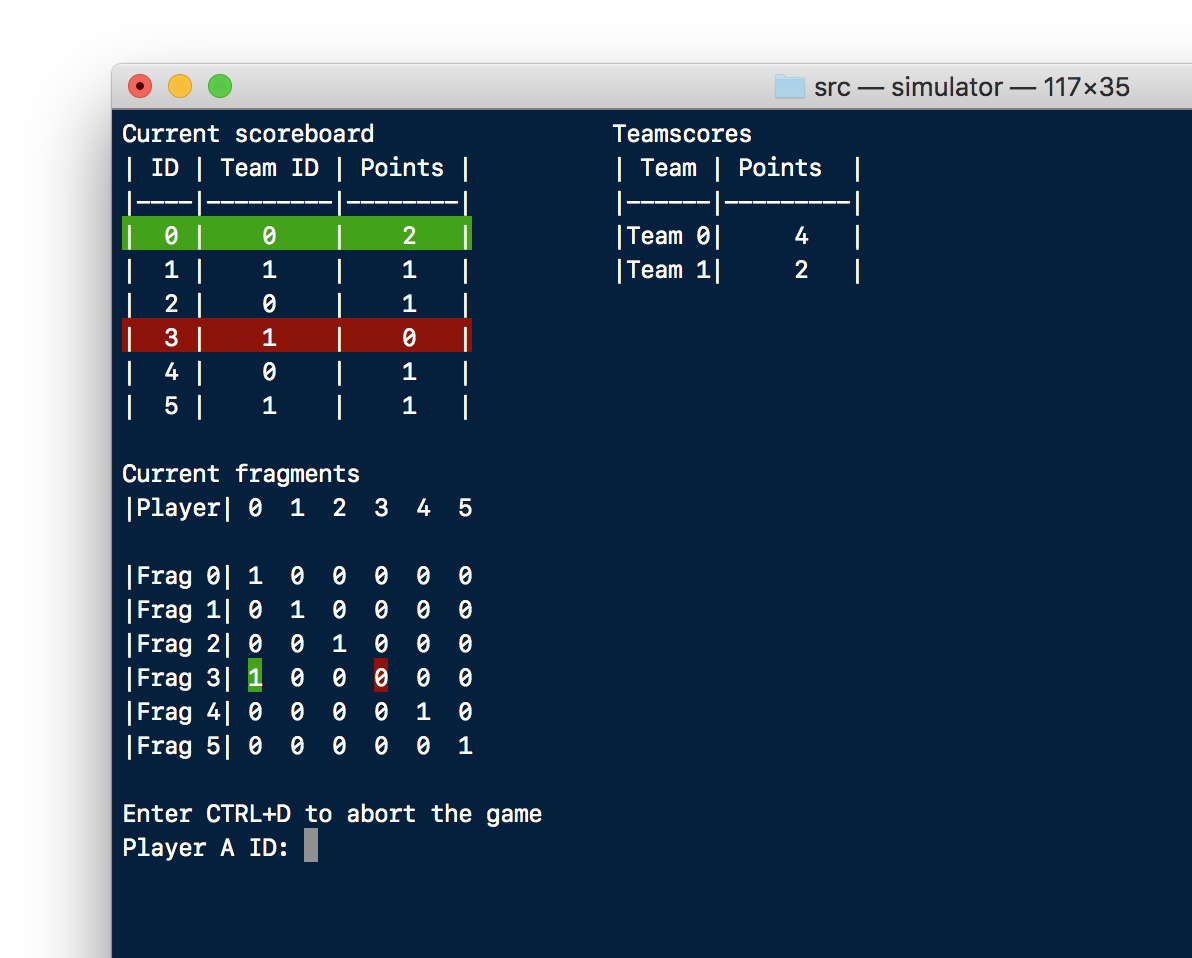
\includegraphics[width=0.7\textwidth,keepaspectratio]{./040-komponenten/030-spielelogik/Simulator.png}
  \caption{Der Simulator}
  \label{fig:simulator}
\end{figure}
Ist ein Spiel gestartet, so können Schüsse simuliert werden, indem jeweils die ID eines Schützen und eines Getroffenen eingegeben wird. Anschließend werden die Veränderungen in Punkten und in den Dateifragmenten jedes Spielers sichtbar. Rot hervorgehobene Zahlen stehen dabei für einen Verlust, grün hervorgehobene Zahlen für einen Gewinn, wie im Bild zu sehen, wie im Bild \cref{fig:simulator} zu sehen.
Am Ende eines Spiels gibt der Simulator den Gewinner (ein Spieler oder ein ganzes Team) aus. \\
Mehr zu den technischen Aspekten des Simulators ist im \cref{sec:api-zu-services-komponente} zu finden.

\paragraph{Solo Easy}
Bei dem Spielmodus „Solo Easy“ handelt es sich um einen Spielmodus, welcher schnell implementiert werden sollte. Demnach soll der Spielmodus einfach spielbar sein. Der Spielmodus funktioniert wie folgt: \\
Jedem Spieler wird ein Dateifragment zugewiesen. Wird ein Spieler durch einen anderen Spieler getroffen, bekommt der Schütze das ursprüngliche Dateifragment des Getroffenen. Dabei ist zu beachten, dass der getroffene Spieler sein Dateifragment jedoch behält, d.h. Dateifragmente werden bei Treffern somit kopiert. Das Spiel endet sobald ein Spieler alle existierenden Dateifragmente besitzt.

\paragraph{Solo Advanced}
Der Spielmodus „Solo Advanced“ baut auf dem Spielmodus „Solo Easy“ auf. Der Unterschied hierbei liegt darin, dass bei einem Treffer der getroffene Spieler sein Dateifragment jedoch nicht behält, d.h. Dateifragmente werden nun bei Treffern abgegeben. Das bedeutet also insbesondere, dass Dateifragmente nicht kopiert werden. Ein Dateifragment zählt hierbei wie ein Punkt. \\
Des Weiteren kann der Spielmodus in mehreren Runden gespielt werden, wobei eine Runde durch ein Zeitlimit begrenzt wird. Eine Runde gewinnt derjenige Spieler, welcher die meisten Punkte, also die meisten Dateifragmente am Ende einer Runde besitzt.

\paragraph{Teams Advanced}
Als Variation kann der Spielmodus „Solo Advanced“ auch teambasiert gespielt werden, wobei die Teamzuweisung manuell erfolgt. Gewonnen hat demnach das Team, welches am Ende einer Runde die meisten Punkte hat. Teambeschuss wird hierbei nicht beachtet (ist nicht erlaubt) und führt demnach zu keinem Ereignis (kein Punktabzug o.Ä.).

\paragraph{No Carry No Win}
„No Carry No Win“ ist ein Spielmodus, der ausschließlich teambasiert gespielt wird, wobei die Teamzuweisung manuell erfolgt. Hierbei wird pro Team ein Spieler zufällig ausgewählt, welcher alle Dateifragmente einer begehrten Datei besitzt, der sogenannten „Carry“. Er hat besondere Bedeutung für das BitTorrent-Netzwerk in dem zugrundeliegenden Szenario, denn da er bereits alle Dateifragmente hat, tritt er nur noch als Seed auf und ist für das Netzwerk (sein Team) besonders wichtig. \\
Nun bricht ein Kampf zwischen den Teams aus, ganz im Stile von Lasertag. In diesem Kampf ist folglich das Ziel jedes normalen Spielers (jedes Spielers, der kein Carry ist), seinen Carry zu verteidigen, ihn also im BitTorrent-Netzwerk zu halten, denn sie wollen von ihm in Zukunft auch noch Dateifragmente erhalten können. \\
Jeder normale Spieler besitzt zu Beginn wie üblich ein Dateifragment. Zu beachten ist hierbei, dass in diesem „Kampf“ Dateifragmente nicht kopiert oder übertragen, sondern nur als Leben gewertet werden. Ein Spieler „stirbt“, scheidet also aus einer Runde aus, wenn er kein Dateifragment mehr besitzt. Das bedeutet, dass ein normaler Spieler nach einem Treffer, der Carry jedoch erst nach mehreren Treffern „stirbt“. \\
Der Spielmodus kann in mehreren Runden gespielt werden, wobei eine Runde dann endet, wenn nur noch ein Carry übrig ist. Das Team, dessen Carry zuletzt übrig ist, gewinnt die jeweilige Runde.
Bei diesem Spielmodus wird ebenfalls kein Teambeschuss toleriert.

\paragraph{Share Or No Share}
Der Spielmodus „Share Or No Share“ soll ein fundamentales Prinzip von BitTorrent besonders hervorheben: die Kollaboration. Jeder neue Peer im Netzwerk profitiert zunächst von den bereits angebotenen Dateifragmenten und sollte anschließend, nach Erhalt des ersten Dateifragments, zur Weiterverteilung der entsprechenden Datei beitragen, indem er seinerseits Dateifragmente anderen Peers zur Verfügung stellt. \\
„Share Or No Share“ wird dafür ausschließlich teambasiert gespielt, wobei die Teamzuweisung zufällig erfolgt. Hierbei werden die Spieler in zwei Teams aufgeteilt, ein faires Team und ein unfaires Team. Wieder wird davon ausgegangen, dass jeder Spieler zu Beginn des Spiels bereits ein Dateifragment erhalten hat. Im fairen Team befinden sich „normale“ Peers, die sowohl Dateifragmente von anderen Peers erhalten als auch selbst Dateifragmente zur Verfügung stellen wollen. Im unfairen Team hingegen befinden sich sogenannte „Power-Leecher“, Peers, die also möglichst schnell alle benötigten Dateifragmente bekommen möchten, jedoch keine zur Verfügung stellen wollen. Die Aufteilung in Teams erfolgt bestmöglich in dem Verhältnis 2:1 (faire:unfaire Spieler), weil uns realistisch erscheint, dass es mehr faire als unfaire Peers gibt. \\
Es gewinnt das Team, welches zum Ende des Spiels die meisten Punkte hat. Dabei werden die Punktzahlen nach \cref{tab:share-or-no-share-punkte} vergeben.
\begin{table}
  \centering
  \begin{tabular}{|c|c|c|}\hline
      trifft & fair & unfair \\ \hline
      fair & $+10$ für beide & $+20$ für Schützen \\
       & & $-20$ für Getroffenen \\ \hline
      unfair & $+20$ für Schützen & $+10$ für Schützen \\
       & $-20$ für Getroffenen & $-10$ für Getroffenen \\ \hline
  \end{tabular}
  \caption{Punktevergabe im Spielmodus „Share Or No Share“ \\
           \footnotesize Zu lesen ist die Tabelle in der Form „\emph{\textless Eintrag aus erste Spalte\textgreater\ trifft \textless Eintrag aus erste Zeile\textgreater}“.}
  \label{tab:share-or-no-share-punkte}
\end{table}
Die Motivation für die Punktzahlen ist wie folgt. Offensichtlich werden Punkte nur auf der fairen Seite „erzeugt“. Das soll unterstreichen, dass BitTorrent prinzipiell nur kollaborativ funktioniert, und nur bei fairem Dateiaustausch ein Mehrwert für alle Peers entsteht. Ansonsten spiegeln die Punktzahlen ganz einfach die Motivation der jeweiligen Spieler wider, entsprechend zu treffen oder getroffen zu werden. So wollen faire Spieler beispielsweise, dass alle anderen Peers im Netzwerk auch fair spielen, also Dateifragmente zur Verfügung stellen. Deshalb bekommen sie mehr Punkte, wenn sie einen unfairen Spieler treffen und ihn damit zum Teilen „zwingen“, als wenn sie einen fairen Spieler treffen. Entsprechend sieht es auf der anderen Seite aus. Unfaire Spieler nutzen also gern die fairen Spieler aus und werden damit mit entsprechend mehr Punkten belohnt. Und für Schüsse innerhalb des unfairen Teams gibt es beim getroffenen unfairen Spieler Punktabzug, weil ein unfairer Spieler mit niemandem „teilen“ möchte. \\
Der Spielmodus hat nur eine Runde, wobei das Spiel endet, sobald ein Spieler alle Dateifragmente gesammelt hat. \\

\noindent
Wir haben die Spielmodi nur mit dem Simulator und nicht im Praxiseinsatz, also auf einem echten Spielfeld mit echten Spielern, testen können. Dadurch könnten uns Faktoren, die den Spielverlauf in der Praxis beeinflussen und damit eventuell Anpassungen an den Annahmen und bspw. Punktzahlen der Spielmodi nötig machen würden, völlig unbekannt geblieben sein. Besonders für das Balancing von Parametern wie Punktzahlen und die Zuweisung der initialen Dateifragmente hätte ein automatisches Testen sinnvoll sein können. Andererseits hätten auch bei automatischen Tests Rahmenbedingungen bzw. Testcases festgelegt werden müssen, die ohne Daten aus der Praxis nur schwer realistisch festgelegt hätten werden können.

Alle drei Mitglieder der Spiellogik Gruppe haben Ideen für Spielmodi vorgeschlagen, die gemeinsam diskutiert wurden. Die Spielmodi „Solo Advanced“ und „Teams Advanced“ sind Ideen von David Bachorska. Der Spielmodus „No Carry No Win“ wurde von Dennis Ness und „Share Or No Share“ von Tom Kieseling entwickelt.
